% Created 2021-01-05 Tue 13:11
% Intended LaTeX compiler: pdflatex
\documentclass{memoir}
\input{/Users/mikevink/.data/nvim/vnnv/latex/preamble.tex}
\usepackage[utf8]{inputenc}
\usepackage[T1]{fontenc}
\usepackage{graphicx}
\usepackage{grffile}
\usepackage{longtable}
\usepackage{wrapfig}
\usepackage{rotating}
\usepackage[normalem]{ulem}
\usepackage{amsmath}
\usepackage{textcomp}
\usepackage{amssymb}
\usepackage{capt-of}
\usepackage{hyperref}
\usepackage{minted}
\author{Mike Vink}
\date{\today}
\title{}
\hypersetup{
 pdfauthor={Mike Vink},
 pdftitle={},
 pdfkeywords={},
 pdfsubject={},
 pdfcreator={Emacs 27.1 (Org mode 9.5)}, 
 pdflang={English}}
\begin{document}

\tableofcontents

\chapterstyle{mike-section}

\chapter{Training command and details}
\label{sec:org9c41d80}

The command I used was mostly adapted from the README file in the sean
directory. The paths to the images and labels were relative paths to the 2000
training images and labels I randomly (seeded) sampled from the CelebA-HQ
dataset. As with SEAN these were cropped to 256x256 during training.

\begin{minted}[breaklines=true,breakanywhere=true]{shell}
python3 train.py --name mike_crop_subset --load_size 256 --crop_size 256 --dataset_mode custom --label_dir path/to/my/train/labels --image_dir path/to/my/train/images --label_nc 19 --no_instance --batchSize 2 --norm_mode clade
\end{minted}

The difference with the SEAN command is that I enabled the CLADE norm\textsubscript{mode}, which is specific to CLADE without it SPADE resblks are used.

\begin{minted}[breaklines=true,breakanywhere=true]{python}
# From CLADE/options/base_options.py
parser.add_argument('--norm_mode', type=str, default='spade', help='[spade | clade]')
\end{minted}

More info on the training process is stored in text files in this directory.

\begin{itemize}
\item \href{fid.txt}{fid scores} only contains two lines. Need to find out when the fid is being
calculated. The options file mentions only that the fid is calculated every 10 epochs.
\item \href{iter.txt}{iter text} also only contains two lines. It is the 45 epochs times 2000
iterations the model has been trained for.
\item \href{loss\_log.txt}{loss log} contains the loss function value per epoch.
\end{itemize}

\section{Continue training}
\label{sec:org2becb53}

I continued training using the following command:

\begin{minted}[breaklines=true,breakanywhere=true]{shell}
python3 train.py --name mike_crop_subset --load_size 256 --crop_size 256 --dataset_mode custom --label_dir path/to/my/train/labels --image_dir path/to/my/train/images --label_nc 19 --no_instance --batchSize 8 --norm_mode clade --tf_log --serial_batches
\end{minted}

I installed the following tenserflow version:

\begin{minted}[breaklines=true,breakanywhere=true]{shell}
pip3 install tensorflow==1.15.0
\end{minted}

After that for some reason I still had to replace in the visualisation utility \texttt{tf} to \texttt{tf.compat.v1}

\begin{minted}[breaklines=true,breakanywhere=true]{python}
# visualiser.py

# search and replace
tf
# to
tf.compat.v1
\end{minted}

When the training was interrupted the out event triggered and the stored iterations were written to a log file.

\section{loss log plots}
\label{sec:orgb0c3c84}

I used the tensorboard log files for this, It should also be able to export the
relevant plots to publication quality images. You can install tensorboard
locally and then google a command to open the log files, or quickly and dirtily
use the command I used:

\begin{minted}[breaklines=true,breakanywhere=true]{shell}
# tensorboard --logdir=/path/to/log_dir
tensorboard --logdir=./mike_crop_subset/logs

# Should open a server where you can see the loss over iterations.
\end{minted}


\chapter{Adverserial loss term}
\label{sec:orgc1ed30b}

The loss function is the same as with the pix2pixHD paper, instead they use a
hinge loss form for the generator loss.

The general GAN loss function in pix2pixHD:

\[
\min_{G} \max_{D} \mathcal{L}(G, D)
\]

we use a multiscale discriminator by default, which you can check in the
multiscale discriminator class in SPADE.

\begin{minted}[breaklines=true,breakanywhere=true]{python}
# From models/networks/discriminator.py
class MultiscaleDiscriminator(BaseNetwork):
    @staticmethod
    def modify_commandline_options(parser, is_train):
        parser.add_argument('--netD_subarch', type=str, default='n_layer',
                            help='architecture of each discriminator')
        parser.add_argument('--num_D', type=int, default=2,
                            help='number of discriminators to be used in multiscale')
        opt, _ = parser.parse_known_args()

        # define properties of each discriminator of the multiscale discriminator
        subnetD = util.find_class_in_module(opt.netD_subarch + 'discriminator',
                                            'models.networks.discriminator')
        subnetD.modify_commandline_options(parser, is_train)

        return parser
# [...]
\end{minted}

So the general loss form is actually (also in SEAN/SPADE),

\[
\min_{E,G} \max_{D_1 , D_2} \sum_{k=1,2}^{} \mathcal{ L }_{GAN}(E,G, D_{k})
\]

which is the minimax game objective. The objective function \(\mathcal{L}\) is given by,

\[
\mathcal{L}_{GAN}(G,D) = \mathbb{E}_{\left( \boldsymbol{s,x}\right)} \left[ \log D(\boldsymbol{s,x}) \right] + \mathbb{E}_{\boldsymbol{s}} \left[ \log(1 - D(\boldsymbol{s} , G(\boldsymbol{s}))) \right]
\]

Where \(s\) is the label map, and \(x\) is the image.

Note that \(D\) is a (set of) fully convolutional network(s) with a sigmoidal activation
function at the end (only in pix2pix paper, or original gan\textsubscript{mode} loss in SPADE
project). This means that the range of \(D\) should be \(\left[ 0,1\right]\).
Where \emph{one} means real and \emph{zero} means fake.

\section{Hinge version\hfill{}\textsc{ATTACH}}
\label{sec:orga9fd9a5}
Now in later papers (SPADE and its derivatives) a hinge form was used, without
any sigmoid predictions. This is best explained in the SEAN paper,

\begin{align}
\mathcal{ L }_{GAN} &= \mathbb{E}_{} \left[ \max(0,1 - D_{k}(\boldsymbol{s,x})) \right] \tag*{\{D\_real\} }\\
 &+ \mathbb{E}_{} \left[ \max(0, 1 + D_{k}(\boldsymbol{s,},G(\boldsymbol{s}))) \right] \tag*{\{D\_fake\} }
\end{align}

Where again \(s\) is the label map and \(x\) is the real image. You can see
that there are two hinge terms, the real and fake discriminator loss. The curly
braces on the right gives how the loss log file refers to these terms. It is
also important to note that these expected values are calculated per mini-batch
\cite{limGeometricGAN2017}. Meaning that low batch size would not accurately
represent the separating hyperplane. But given enough time it still would find
an optimum.

We also have two-scale discriminators, so the value reported in loss$\backslash$\textsubscript{log.txt} is
actually the mean of the two

This is equivalent to the following (Zhang et al. 2019: SAGAN):

\begin{align}
\mathcal{ L }_{D} &= - \mathbb{E}_{(\boldsymbol{s,x})} \left[ \min(0, -1 + D(\boldsymbol{s,x})) \right] \tag*{\{D\_real\} }\\
 &- \mathbb{E}_{s} \left[ \min(0, -1 - D(G(\boldsymbol{s}) , \boldsymbol{s})) \right] \tag*{\{D\_fake\} }\\
\mathcal{ L }_{G} &= - \mathbb{E}_{\boldsymbol{s} } \left[ D(G(\boldsymbol{s}) , \boldsymbol{s}) \right] \tag*{\{GAN\} }
\end{align}

Where \(\mathcal{ L }_{G}\) is the generator loss, this is important, because
we are training stepwise the generator and discriminator. One step the
\(\mathcal{ L }_{D}\) is computed and \(\mathcal{ L }_{G}\) in the other.


It can be shown that this equation converges to \(2\) , and that is equivalent
to pushing the generated image to the separating hyperplane, and optimising the
hyperplane margins for the discriminator (geometric gan paper).

The intuition for this is that when the probability distribution of the real
images and fake images are equivalent, or the reverse KL-divergence \(KL \left[ p_{g} || q_{data}\right]\)
is minimised \cite{miyatoSpectralNormalizationGenerative2018}. Especially the
example of learning parallel lines at the end of section 3 of the paper was
nice. The paper also gives the geometric intuition for the hinge loss



\begin{center}
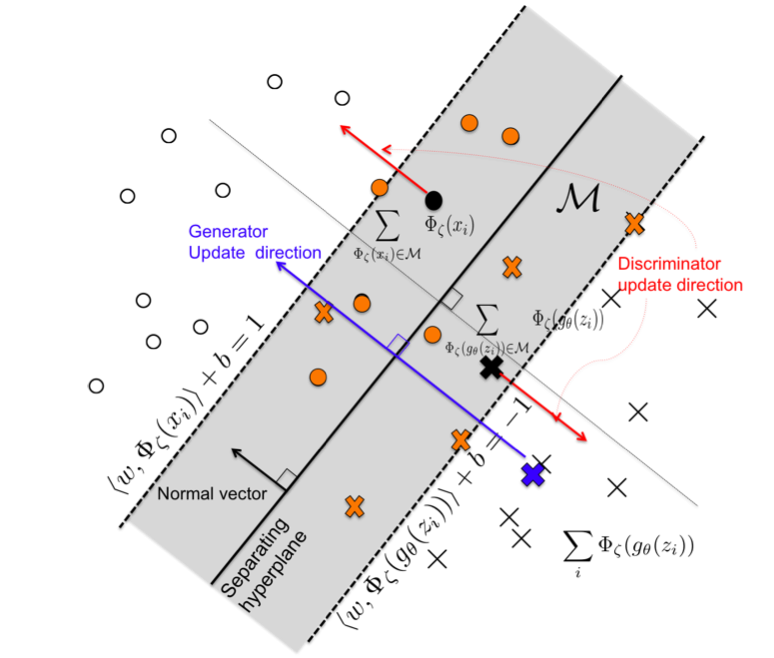
\includegraphics[width=.9\linewidth]{/Users/mikevink/Documents/python/pr_project/CLADE/checkpoints/mike_crop_subset/figs/_20210104_131213Screenshot 2021-01-04 at 13.11.45.png}
\end{center}

As you can see the discriminator tries to push away from the hyperplane where \(D = 0\),
and the generator tries to push towards the \(0\) .


\bibliographystyle{unsrt}
\bibliography{../../../../../../Dropbox/bibliography/references}
\end{document}
